\documentclass{article}
\usepackage{mathtools}
\usepackage{graphicx}
\begin{document}
	\section*{Lsg Vorschlag A+N Ü009 Maximilian Maag}
	\section*{Aufgabe A}
	$sinh(x) = \frac{1}{2}*(e^x - e^{-x})$ \\
	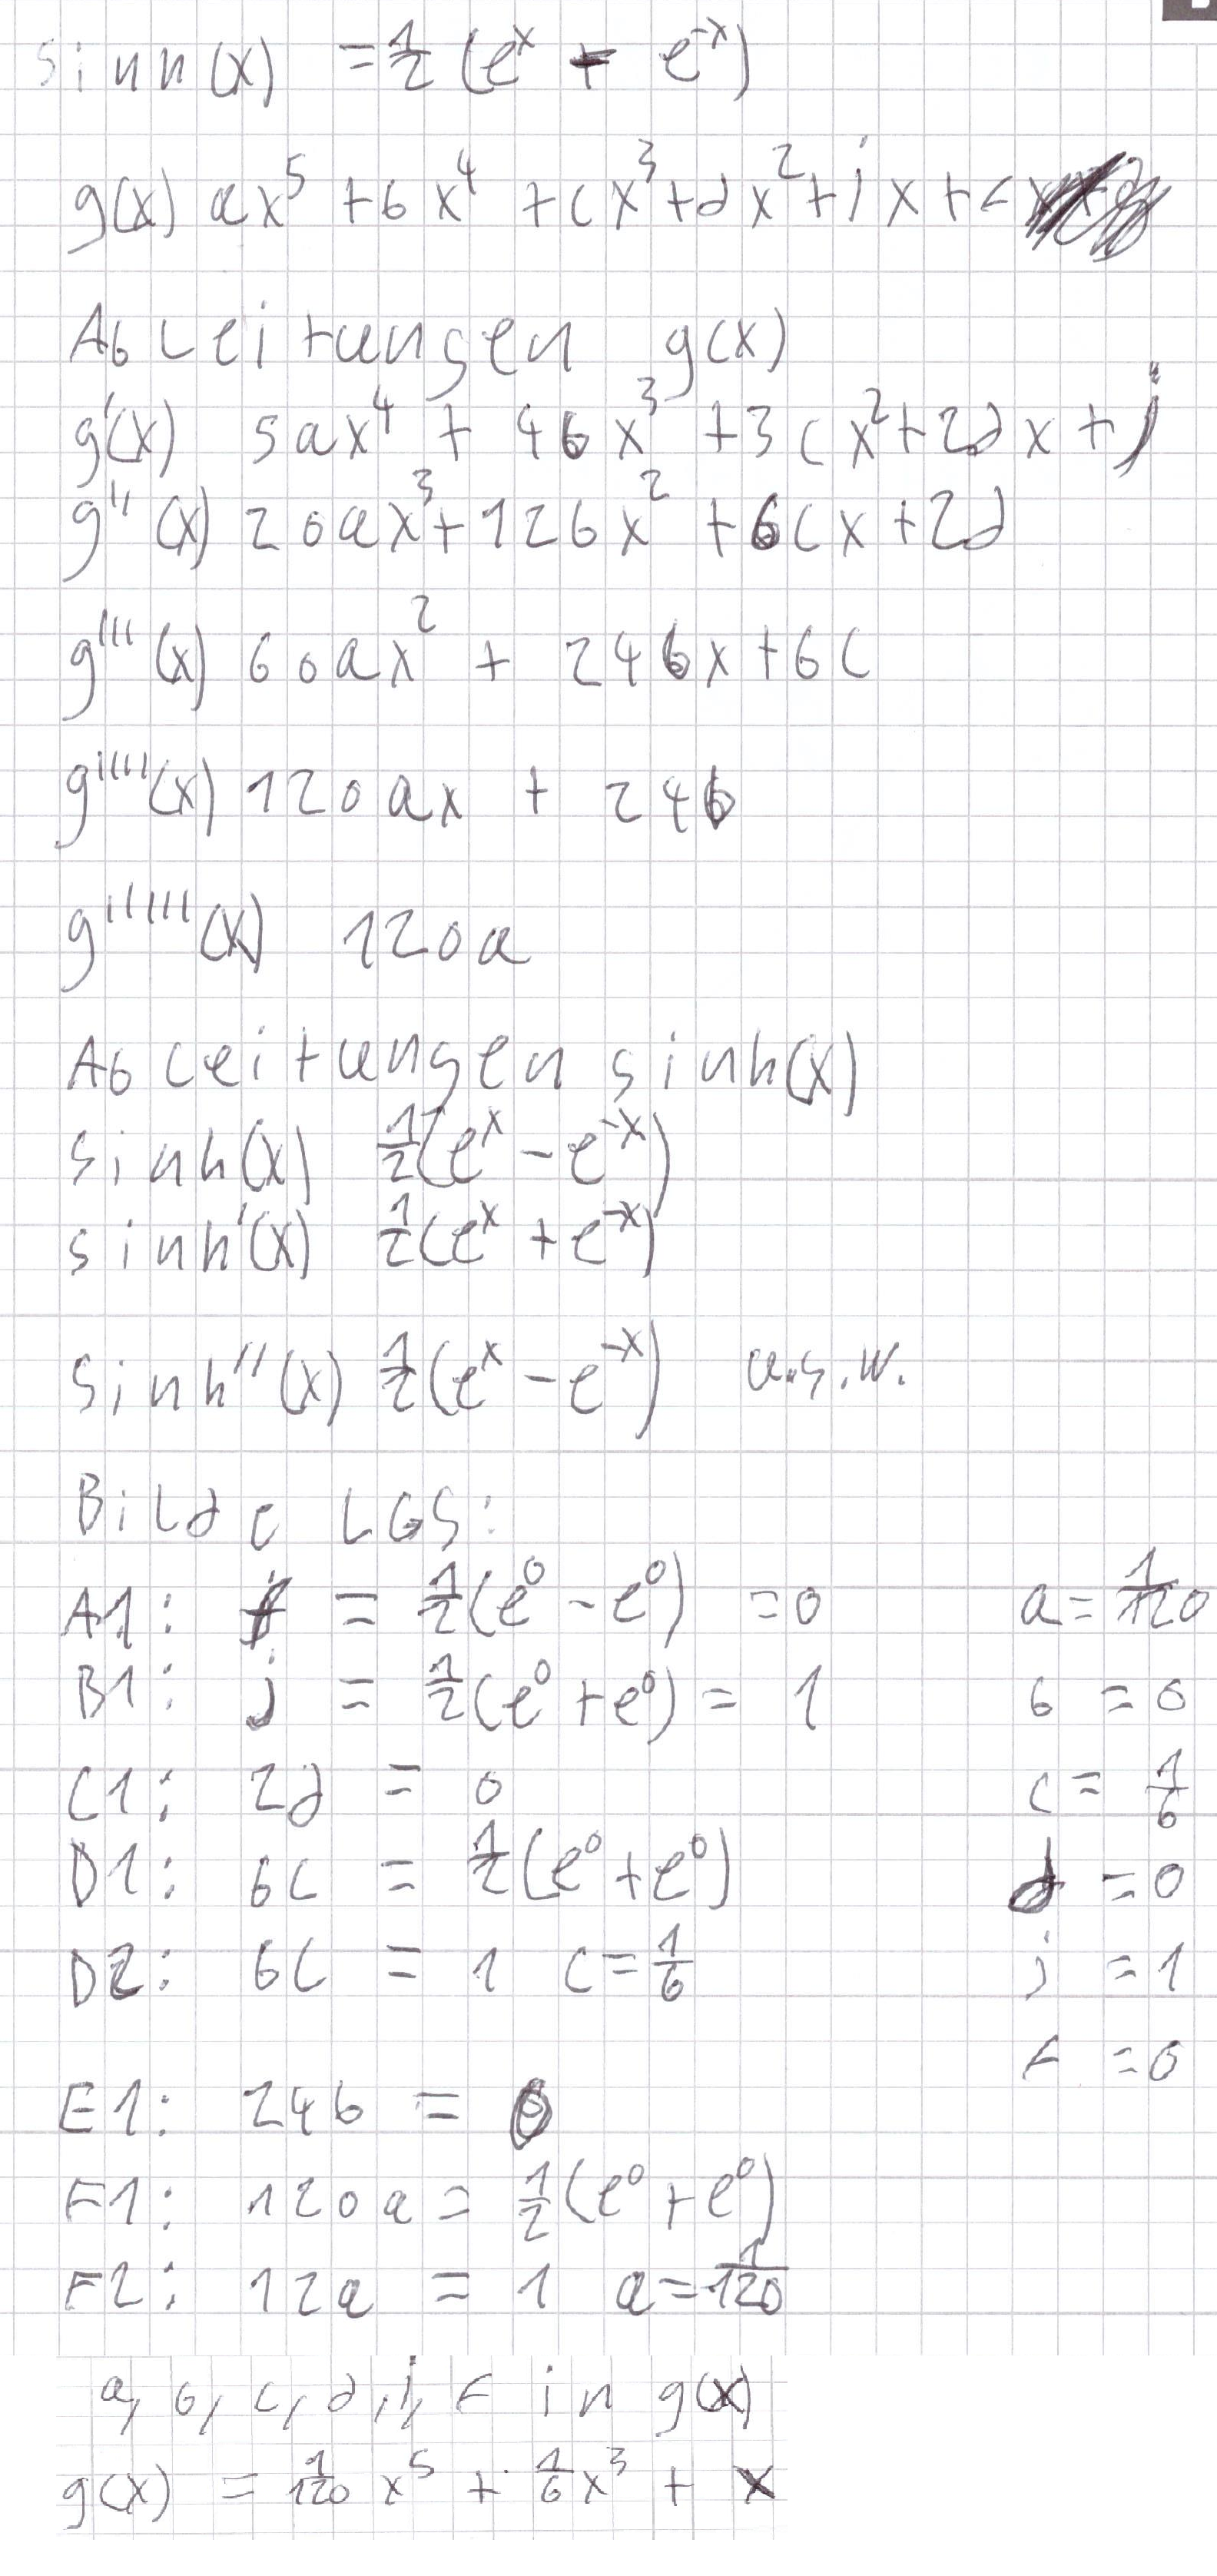
\includegraphics[height=\linewidth, width=\linewidth]{9A} \\
	$g(x) = \frac{1}{120}x^5 + \frac{1}{6}x^3 + x$
	\section*{Aufgabe B}
	Ansatz nach Newton: \\
	$f(x) = a + b(x-0) + c(x-0)(x-1) + d(x-0)(x-1)(x-2)$ \\
	\\
	A: $a = 1$ \\
	B: $a + b = 2$ \\
	C: $a + 2b + 2c = 9$ \\
	a = 1; b = 1; c = 3 \\
	in f(x) \\
	$f(x) = 1 + x + 3(x-0)(x-1)$ \\
	$f(x) = 1 + x + 3x(x-1)$ \\
	$f(x) = 1 + x + 3x^2 -3x$ \\
	$f(x) = 3x^2 -2x + 1$ \\
	\section*{Aufgabe 1}
	\subsection*{a)}
	$f(x) = 3e^{-\frac{1}{2}x}$ \\
	Ansatz nach Taylor: \\
	$g(x) = ax^2 + bx + c$ \\ 
	soll die Funktion f approximieren. \\ \\
	Bedingungen: \\
	$f(0) = g(0)$ \\
	$f'(0) = g'(0)$ \\
	$f''(0) = g''(0)$ \\
	\\
	Ableitungen g(x): \\
	$g'(x) = 2ax + b$ \\
	$g''(x) = 2a$ \\ \\
	Ableitungen f(x): \\
	$f'(x) = 3 * (-\frac{1}{2})*e^{-\frac{1}{2}x}$ \\
	$f'(x) = -\frac{3}{2}*e^{-\frac{1}{2}x}$ \\
	$f''(x) = \frac{3}{4}*e^{-\frac{1}{2}x}$ \\ \\ \\
	Aus Bedingungen resultiert LGS \\
	A: $a*0^2 + b*0 + c = 3e^{-\frac{1}{2}*0}$ \\
	B: $ 2a*0 + b = -\frac{3}{2}*e^{-\frac{1}{2}*0}$ \\
	C: $ 2a = \frac{3}{4}*e^{-\frac{1}{2}*0}$ \\ \\
	A1: $c = 3e^{0}$ \\
	B1: $b = -\frac{3}{2}*e^{0}$ \\
	C1: $2a = \frac{3}{4}*e^{0}$ \\ \\
	Aus $e^0 = 1$ ergibt sich:\\
	A2: $c = 3$ \\
	B2: $b = -\frac{3}{2}$ \\
	C2: $2a = \frac{3}{4}$ \\
	C3: $a = \frac{3}{8}$ \\
	a, b und c in g(x) ergibt:
	$g(x) = \frac{3}{8}x^2 - \frac{3}{2}x + 3$ an der Entwicklungsstelle 0.
	\subsection*{b)}
	\section*{Aufgabe 2}
	$cosh(x) = \frac{1}{2}(e^x + e^{-x})$ \\
	
	\subsection*{a)}
	Ansatz nach Taylor für Taylorpolynom 6. Ordnung \\
	$g(x) = ax^6 + bx^5 + cx^4 + dx^3 + jx^2 + fx + g$ \\ \\
	$sinh(0) = g(x)$ \\
	$sinh'(0) = g'(0)$ \\
	$sinh''(0) = g''(0)$ \\
	$sinh'''(0) = g'''(0)$ \\
	$sinh''''(0) = g''''(0)$ \\
	$sinh'''''(0) = g'''''(0)$ \\
	$sinh''''''(0) = g''''''(0)$ \\	\\
	Ableitungen g(x) \\
	$g(x) = ax^6 + bx^5 + cx^4 + dx^3 + jx^2 + fx + g$ \\
	$g'(x) = 6ax^5 + 5bx^4 + 4cx^3 + 3dx^2 + 2jx + f$ \\
	$g''(x) = 30ax^4 + 20bx^3 + 12cx^2 + 6dx + 2j$ \\
	$g'''(x) = 120ax^3 + 60bx^2 + 24cx + 6d$ \\
	$g''''(x) = 360ax^2 + 120bx + 24c$ \\
	$g'''''(x) = 720ax + 120b$ \\
	$g''''''(x) = 720a$ \\ \\
	Ableitungen cosh(x) \\
	$cosh(x) = \frac{1}{2}(e^x + e^{-x})$ \\
	$cosh(x) = \frac{1}{2}e^x + \frac{1}{2}e^{-x}$ \\
	$cosh'(x) = \frac{1}{2}e^x*1 + \frac{1}{2}e^{-x}*-1$ \\
	$cosh'(x) = \frac{1}{2}(e^x - e^{-x})$ \\
	$cosh''(x) = \frac{1}{2}(e^x + e^{-x})$ \\
	$cosh'''(x) = \frac{1}{2}(e^x - e^{-x})$ \\
	$cosh''''(x) = \frac{1}{2}(e^x + e^{-x})$ \\
	$cosh'''''(x) = \frac{1}{2}(e^x - e^{-x})$ \\
	$cosh''''''(x) = \frac{1}{2}(e^x + e^{-x})$ \\ \\ \\ \\
	Bilde LGS mit Tayloransatz: \\
	A1: $g = \frac{1}{2}(e^0 + e^0) = 1$  \\
	B1: $f = \frac{1}{2}(e^0 - e^0) = 0 $ \\
	C1: $ 2j = \frac{1}{2}(e^0 + e^0)$ \\
	C2: $j = \frac{1}{2}$ \\
	D1: $6d = \frac{1}{2}(e^0 - e^0)$\\
	D2: $d = 0$\\
	E1: $24c = \frac{1}{2}(e^0 + e^0)$\\
	E2: $c = \frac{1}{24}$ \\
	F1: $120b =  \frac{1}{2}(e^0 - e^0)$ \\
	F2: $b = 0$ \\
	G1: $720a =  \frac{1}{2}(e^0 + e^0) $\\
	G2: $720a =  1 $\\
	G3: $a = \frac{1}{720} $\\
	$a = \frac{1}{720}$; $b = 0$; $c = \frac{1}{24}$; $d = 0$; $j = \frac{1}{2}$; $f = 0$; $g = 1$ \\ \\
	in g(x) \\
	$g(x) =  \frac{1}{720}x^6  + \frac{1}{24}x^4 + \frac{1}{2}x^2 + 1$
	\subsection*{b)}
	\subsection*{c)}
	\section*{Aufgabe 3}
	\subsection*{a)}
	Ansatz für Stützpolynom nach Newton: \\
	(1,1); (3,4); (5,9) \\
	$f(x) = a + b(x-1) + c(x-1)(x-3) + d(x-1)(x-3)(x-5)$ \\ \\
	LGS bilden: \\
	A: $a = 1$ \\
	B: $a + 2b  = 4$ \\
	C: $a + 4b + 6c = 9$ \\
	$a = 1$, $b = \frac{3}{2}$, $c = \frac{1}{3}$ \\ \\
	in f(x) \\
	$f(x) = 1 + \frac{3}{2}(x-1) + \frac{1}{3}(x-1)(x-3)$ \\
	\subsection*{b)}
	(1,1); (3,4); (5,9); (4,6) \\
	$f(x) = a + b(x-1) + c(x-1)(x-3) + d(x-1)(x-3)(x-5)$ \\ \\
	LGS bilden: \\
	A: $a = 1$ \\
	B: $a + 2b  = 4$ \\
	C: $a + 4b + 6c = 9$ \\
	D: $a + 3b + 4c + 3d = 6$ \\
	B2: $1 + 2b  = 4$ \\
	B3: $b  = \frac{3}{2}$ \\
	C2: $1 + 4*\frac{3}{2} + 6c = 9$ \\
	C3: $7 + 6c = 9$ \\
	C3: $c = \frac{1}{3}$ \\
	D2: $1 + \frac{9}{2} + \frac{4}{3} + 3d = 6$ \\
	D3: $1 + \frac{54}{12} + \frac{16}{12} + 3d = 6$ \\
	D4: $3d = 6 - \frac{54}{12} - \frac{16}{12} - \frac{12}{12}$ \\
	D5: $3d = \frac{72}{12} - \frac{54}{12} - \frac{16}{12} - \frac{12}{12}$ \\
	D6: $3d = -\frac{10}{12}$ \\
	D6: $d = -\frac{10}{36}$ \\ \\
	$f(x) = 1 + \frac{3}{2}(x-1) + \frac{1}{3}(x-1)(x-3) - \frac{10}{36}(x-1)(x-3)(x-5)$
\end{document}